% !Mode:: "TeX:UTF-8"%確保文檔utf-8編碼
\documentclass[tikz,border=2pt]{standalone}
\usepackage{pgfplots}
\pgfplotsset{compat=newest}
\begin{document}
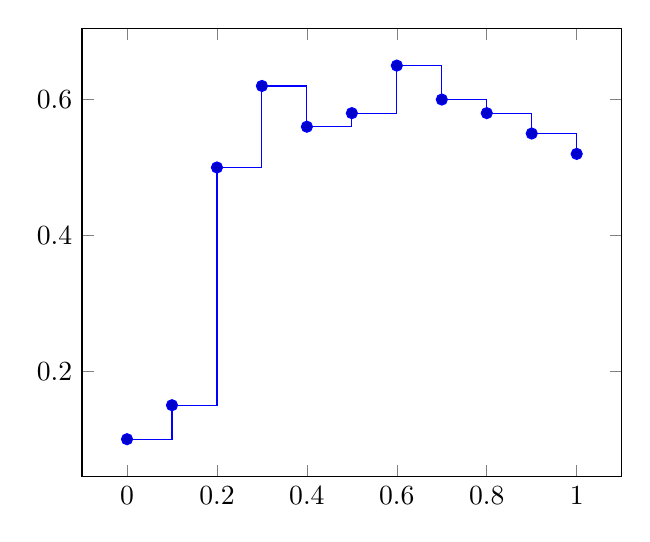
\begin{tikzpicture}
\begin{axis}
\addplot+[const plot]
coordinates
{(0,0.1)    (0.1,0.15)  (0.2,0.5)   (0.3,0.62)
 (0.4,0.56) (0.5,0.58)  (0.6,0.65)  (0.7,0.6)
 (0.8,0.58) (0.9,0.55)  (1,0.52)};
\end{axis}
\end{tikzpicture}

\begin{tikzpicture}
\begin{axis}
	\addplot+[sharp plot] coordinates 
		{(0,0) (1,2) (2,3)};
\end{axis}
\end{tikzpicture}


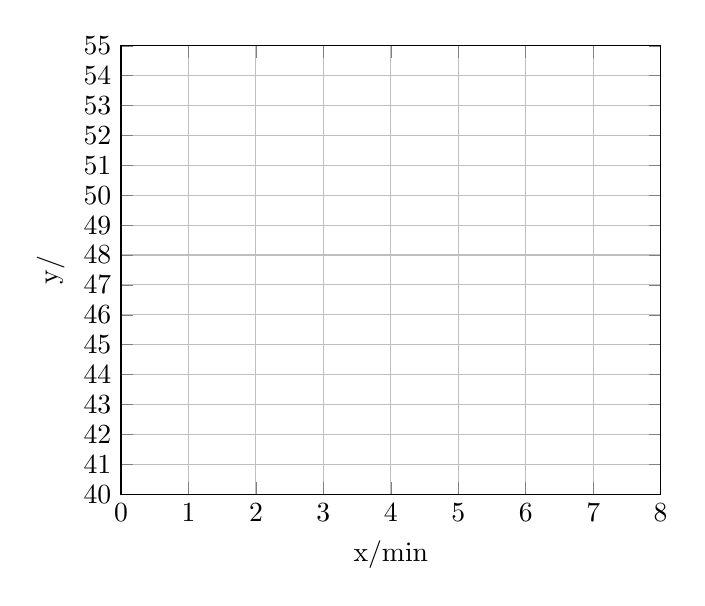
\begin{tikzpicture}
\begin{axis}[
xlabel=x/min,
ylabel=y/,
xmin=0,
xmax=8,
ymin=40,
ymax=55,
grid=major,
xtick={0,1,2,3,4,5,6,7,8},
ytick={40,41,42,43,44,45,46,47,48,49,50,51,52,53,54,55}]
\addplot[mark=x] coordinates {
};
\end{axis}
\end{tikzpicture}


\usepgfplotslibrary{polar}

\begin{tikzpicture}
	\begin{polaraxis}
	\addplot coordinates {(0,1) (90,1) 
		(180,1) (270,1)};
	\end{polaraxis}
\end{tikzpicture}










\usepgfplotslibrary{ternary}

\begin{tikzpicture}
\begin{ternaryaxis}[
	title=Want--be--Stainless Steel,
	xlabel=Weight Percent Chromium,
	ylabel=Weight Percent Iron,
	zlabel=Weight Percent Nickel,
	label style=sloped,
	area style,
]
	\addplot3 table {
	A B C
	1 0 0
	0.5 0.4 0.1
	0.45 0.52 0.03
	0.36 0.6 0.04
	0.1 0.9 0
	};
	\addlegendentry{Cr}

	\addplot3 table {
	A B C
	1 0 0
	0.5 0.4 0.1
	0.28 0.35 0.37
	0.4 0 0.6
	};
	\addlegendentry{Cr+$\gamma$FeNi}

	\addplot3 table {
	0.4 0 0.6
	0.28 0.35 0.37
	0.25 0.6 0.15
	0.1 0.9 0
	0 1 0
	0 0 1
	};
	\addlegendentry{$\gamma$FeNi}

	\addplot3 table {
	0.1 0.9 0
	0.36 0.6 0.04
	0.25 0.6 0.15
	};
	\addlegendentry{Cr+$\gamma$FeNi}

	\addplot3 table {
	0.5 0.4 0.1
	0.45 0.52 0.03
	0.36 0.6 0.04
	0.25 0.6 0.15
	0.28 0.35 0.37
	};
	\addlegendentry{$\sigma$+$\gamma$FeNi}

	\node[inner sep=0.5pt,circle,draw,fill=white,pin=-15:\footnotesize Stainless Steel] 
	  at (axis cs:0.18,0.74,0.08) {};
	
\end{ternaryaxis}
\end{tikzpicture}




\begin{tikzpicture}
\begin{axis}
	\addplot+[smooth] coordinates 
		{(0,0) (1,2) (2,3)};
\end{axis}
\end{tikzpicture}




\usepgfplotslibrary{units}
\begin{tikzpicture}
  \begin{axis}[change x base,
    x SI prefix=kilo,x unit=m,
    y SI prefix=milli,y unit=N,
    xlabel=Distance,ylabel=Force]
    \addplot coordinates {
        (1000,1)
        (2000,1.1)
        (3000,1.2)
        (4000,1.3)
    };
  \end{axis}
\end{tikzpicture}






\end{document}